\chapter{Avaliação dos Resultados}
\label{cap:impl}
De forma a avaliar a implementação desenvolvida, foi selecionado o tópico:
\textit{``Canada will welcome you, Trudeau invites refugees as Trump bans
them''.}
A partir desse tópico, foram extraídos comentários que foram avaliados de
forma manual. Após, esses comentários foram processados através da ferramenta
\ac{NLTK}, obtendo uma assertividade de 56\%.

Observa-se que uma grande parte dos comentários que foram identificados de forma
incorreta apresentam irônia, como por exemplo: \textit{``lol Good Luck
Canada''}. A identificação de ironia através da leitura textual se
faz difícil até mesmo para um ser-humano uma vez que o texto pode
não apresentar sinais de humor. De fato, no caso de comentários
irônicos como \textit{``Good luck with that.''} e suas variações, que aparecem
trinta vezes no tópico selecionado, a metologia de análise de sentimentos se
apresenta falha. A ironia para a análise de sentimentos é considerado
um tópico problemático sendo alvo de diversos estudos \cite{DBLP:conf/lrec/StranisciBFP16}.

Já para outros comentários que foram identificados de forma incorreta
observa-se que o sentimento expresso não se encontrava em dicionário de
sentimentos padrão do \ac{VADER}. De forma a minimizar este problema, foi
utilizado o método de Propagação Dupla, que apresenta-se com o objetivo de
adicionar novas palavras ao dicionário \cite{Qiu:2011:OWE:1970420.1970422}.

\section{Método de Propagação Dupla}

O método de Propagação Dupla, proposto por Qiu
\cite{Qiu:2011:OWE:1970420.1970422}, apresenta como objetivo resolver dois
problemas do \ac{NLP}, que são a expansão do dicionário e também a extração de
alvos dos comentários. Os \textit{``Opinion targets"} ou alvos de opinião, são
palavras as quais sentimentos se referem. Por exemplo, na frase ``Essa
música é muito boa", a palavra ``boa'' demonstra o sentimento do autor com relação a
``música''. Tornando assim, a palavra música um alvo de opinião. 

A extração dos alvos se faz necessária uma vez que, em determinadas frases
podemos ter várias opiniões expressas sobre diversos alvos. Além disso, podemos
ter opiniões diferentes sobre diferentes características de algo. Por exemplo, na frase ``Este celular é muito bom, porém a bateria dele é péssima", tem-se que o
produto em si é bom, porém, a opinião sobre a bateria dele é negativa. De
forma, a resolver esse problema, novas palavras e alvos são adicionados ao
dicionário a partir da execução das quatro tarefas que serão descritas na
próxima seção.

\subsection{Adição de Palavras e Alvos ao Dicionário}

A primeira tarefa, é dividida em duas regras, sendo que a primeira regra será a
extração de alvos a partir de palavras que expressam sentimentos e que já são
conhecidas. Ou seja, são verificadas todas as palavras das quais a palavra que
expressa sentimentos depende. Caso essa palavra seja um substantivo, ela será
extraída e adicionada na lista de alvos de sentimentos. Por exemplo na frase \textit{``We have a great president''} a palavra \textit{``great''} depende de \textit{``president''}, que é um substantivo. Neste caso, a palavra \textit{``president''} será adicionada a
lista de alvos de sentimentos.

\[\textit{We have a } \underbrace{\textit{great president.}}_\text{president
\textrightarrow \text{ great}}\]

A segunda regra da primeira tarefa,
verifica se uma palavra que expressa sentimentos é dependente de uma segunda
palavra que depende de um substantivo.
Por exemplo, na frase \textit{``Trump is a great president.''} a palavra
\textit{``great''} depende da palavra \textit{``is''} que por sua vez depende da
palavra \textit{``president''} que é um substantivo. Neste caso, a palavra
\textit{``president''} será adicionada a lista de palavras que são alvos de sentimentos.

\[\textit{Trump} \underbrace{\textit{is a great president.}}_\text{president
\textrightarrow \text{ is} \textrightarrow \text{ great}}\]

A segunda tarefa é a extração de novas palavras que expressam sentimentos. Para isso, são utilizadas duas
regras. Na primeira regra, é verificada se a frase alguma palavra que se
encontra na lista de alvos de sentimentos, em caso positivo, é verificado se
essa palavra possui algum dependente que seja um adjetivo. Por exemplo, na frase \textit{``Trump is a witty president.''}, a palavra \textit{``president''} foi
extraída na tarefa anterior, porém, a palavra \textit{``witty''} ainda não se
encontra no dicionário de sentmientos.
Ao processar a segunda tarefa, a palavra \textit{``witty''} será acrescida ao
dicionário de sentimentos uma vez que essa palavra é um adjetivo e que ainda não
existe no dicionário.


\[\textit{We have a } \underbrace{\textit{witty president.}}_\text{president
\textrightarrow \text{ witty}}\]

A segunda regra da segunda tarefa 
verifica se uma palavra alvo possui um dependente, que por sua vez possui um
adjetivo como dependente. Por exemplo, na frase
\textit{``Trump is a witty president.''} a palavra \textit{``witty''}, que é um
adjetivo, depende de \textit{``is''} que por sua vez depende de
\textit{``president''}. Neste caso, a palavra \textit{``witty''}
será acrescida ao dicionário de sentimentos uma vez que essa é um adjetivo que
não existe ainda no dicionário.

\[\textit{Trump} \underbrace{\textit{is a witty president.}}_\text{president
\textrightarrow \text{ is} \textrightarrow \text{ witty}}\]

A terceira tarefa é a extração de palavras alvo a partir de palavras alvo que
foram extraídas anteriormente. A primeira regra desta tarefa verifica se a frase
possui alguma palavra na lista de alvos, e verifica se essa possui alguma
conjunção. Em caso positivo, a palavra após a conjunção é adicionada na lista
de alvos. Por exemplo, na frase \textit{``We have a great president and
leader."}, a palavra \textit{``president''} que foi extraída através
da primeira tarefa, possui a conjunção \textit{``and''} que a relaciona com a
palavra \textit{``leader''}, a qual não consta na lista de palavras alvo. Neste
caso, a palavra \textit{``leader''} será adicionada a lista de palavras alvo.


\[\textit{We have a great} \underbrace{\textit{president and
leader.}}_\text{president \textrightarrow \text{ and} \textrightarrow \text{
leader}}\]

A segunda regra da terceira tarefa verifica se dois substantivos
possuem uma palavra dependente em comum. No caso de um desses substantivos ser
uma palavra alvo, o outro também é adicionado na lista. Por exemplo, na frase
\textit{``Trump is a great president.''}, a palavra \textit{``president''} que
foi extraída através da primeira tarefa possui a palavra \textit{``is''} como
dependente, bem como a palavra ``Trump'' também possui a palavra \textit{``is''}
como dependente. Desta forma, a palavra \textit{``Trump''} será adicionada a
lista de alvos.

\[\underbrace{\textit{Trump is a great president.}}_\text{Trump
\textrightarrow \text{ is} \textleftarrow \text{ president}}\]



A última tarefa tem como objetivo a extração de novas opiniões a partir de
adjetivos já extraídos. A primeira regra desta tarefa, efetua a extração através
das conjunções presentes no texto. Por exemplo, para a frase \textit{``Trump is
witty and clever.''}, a palavra \textit{``witty''} possui uma conjunção
(\textit{``and''}), relacionando a palavra \textit{``clever''}. Neste caso, será
extraída a palavra \textit{``clever''} e adicionada no dicionário.

\[\textit{Trump} \underbrace{\textit{is witty and clever.}}_\text{witty
\textleftarrow \text{ and} \textrightarrow \text{ clever}}\]


Na última regra da tarefa quatro, é verificado-se dois adjetivos
dependem de uma mesma palavra. Se uma destas palavras pertence ao dicionário de
sentimentos, a outra também será adicionada na lista. Por exemplo, na frase
\textit{``Trump is witty, clever''}, ambas as palavras \textit{``witty''} e
\textit{``clever''} dependem de \textit{``Trump''}. Neste caso, será extraída a
palavra \textit{``clever''} e adicionada ao dicionário.

\[\textit{Trump} \underbrace{\textit{is witty, clever.}}_\text{witty
\textleftarrow \text{ Trump} \textrightarrow \text{ clever}}\]

Por fim, é verificado se o número de palavras da lista de alvos ou sentimentos
aumentou. Em caso positivo, as quatro tarefas serão executadas até que nenhuma palavra seja acrescentada a
uma das listas.

\subsection{Atribuição de Pontuação às Novas Palavras}
A pontuação das novas palavras do dicionário de sentimentos é realizada
considerando-se: para as palavras extraídas através da quarta tarefa, é
utilizada a mesma pontuação da palavra relacionada a essa nova palavra. Para palavras extraídas através da segunda tarefa é utilizada a mesma pontuação
da palavra utilizada para a extração do alvo a qual essa palavra utiliza. Por
exemplo, na primeira regra foi extraída a palavra \textit{``president''} a
partir de \textit{``great''}. Desta forma, será atribuido para a palavra
\textit{``president''} a mesma pontuação da palavra \textit{``witty''}. Como por
exemplo no comentário \textit{``This president is witty.''}, na
segunda tarefa, a palavra \textit{``witty''}, que foi extraída através de \textit{``president''}, irá receber a mesma pontuação da palavra \textit{``great''}.

Como visto, para utilização do método de Propagação Dupla, é necessário um
conjunto de textos para que sejam executadas as quatro tarefas. Segundo Qiu
\cite{Qiu:2011:OWE:1970420.1970422}, como as palavras tem diferentes
significados em diferentes contextos, é recomendado que este conjunto de textos
pertença ao mesmo contexto que está sendo efetuada a análise de sentimentos. Por
exemplo, ao utilizar um conjunto de dados sobre notícias gerais, pode-se
determinar que a palavra \textit{``gucci''} é uma gíria similar a palavra
\textit{``good''}, porém, ao utilizar essa mesma palavra em um contexto de
avaliação de roupas para a análise de sentimentos, pode ser prejudicada a
análise, visto que neste contexto a palavra \textit{``Gucci''} é referente ao produto e não a gíria.

A fim de se determinar o
melhor conjunto de textos para utilização do método, foram utilizados dois
conjuntos de dados diferentes. No primeiro conjunto de textos, consideramos como
contexto outros comentários do mesmo usuário que está sendo efetuada a análise
de sentimentos. Para o segundo conjunto de textos, foram considerados
comentários de usuários em outros tópicos seguindo o mesmo tema. Neste
avaliação, foram utilizados os comentários presentes nos tópicos de política
internacional descritos através do Capítulo 4.3.
 
Após a utilização do Método de Propagação Dupla, utilizando os dois conjuntos
de textos e a avaliação dos comentários foram
obtidos os seguintes resultados a partir do tópico \textit{``Canada will welcome
you,” Trudeau invites refugees as Trump bans them}:
\begin{itemize}
  \item 58\% de assertividade na utilização do dicionário padrão.
  \item 59\% de assertividade na utilização do dicionário padrão com palavras
  extraídas a partir de comentários do mesmo autor.
  \item 62\% de assertividade na utilização do dicionário padrão com palavras
  extraídas a partir de comentários de um mesmo tema.
\end{itemize}
 
Destaca-se que mesmo com o aumento na assertividade com a utilização de
comentários de tópicos do mesmo domínio, os comentários que não foram
identificados de forma correta são comentários como: \textit{"...These
laws are not "racist", morons keep hysterically throwing that word around and
its losing all meaning..."}, aonde que o sentimento expresso é negativo, porém,
a pessoa expressa um sentimento a favor da notícia em questão. 

Para a solução deste problema, são extraídos somente os sentimentos relacionados
com uma palavra determinada de maneira que o sentimento indicado pelo programa
esteja isolado de outras palavras também alvos de sentimento. Por exemplo, no
tópico: \textit{``Canada will welcome
you,” Trudeau invites refugees as Trump bans them} temos sentimentos expressos
com relação ao Trump, Trudeau, Canada e os refugiados, de forma que, somente
efetuando a leitura do comentário em questão, é possível a se determinar sobre o
que aquele comentário positivo ou negativo se refere. 

Ao analisarmos somente a relação de dependência da palavra que se quer saber o
sentimento do comentário, é possível se determinar de forma mais precisa qual o
sentimento do usuário com relação ao assunto escolhido, eliminando outros
sentimentos expressos relacionados com outros alvos ou assuntos. Por exemplo,
no comentário: \textit{``Come enjoy our 15% tax :D
edit: Trudeau is the most fake person ever. He always pulls this shit but
undercuts us Canadians all the time. He ain't getting voted in next
election.''}, a primeira frase apresenta um sentimento positivo, mesmo que de
forma irônica, porém, o resto do texto apresenta um sentimento negativo.
Analisando somente as palavras dependentes de ``Trudeau", somente a frase
\textit{``\ldots is the most fake person ever''} será analisada, demonstrando o
real sentimento do comentário com relação a ``Trudeau'', que é negativo.

Utilizando a palavra ``Trump'' para extração dos comentários do tópico \textit{``Canada will welcome
you,” Trudeau invites refugees as Trump bans them}, foi obtida a assertividade
de 65\%.


\subsection{Uso da Ferramenta para Análise de
Sentimentos na Rede Social Reddit}

A partir da ferramenta desenvolvida, foi realizada a análise dos tópicos
descritos através do Capítulo 4.3, utilizando um dicionário gerado através do
Método de Propagação Dupla com palavra extraídas de um mesmo tema, e também
foram escolhidas palavras alvo para extração dos comentários e sentimentos
relacionados com elas. A partir deste processo, foram obtidos os seguintes
resultados:

\begin{itemize}
  \item 75\% de assertividade no tópico \textit{Official Discussion - mother!}.
  \item 72,34\% de assertividade no tópico \textit{Official Discussion: Gerald's
  Game}.
  \item 63,04\% de assertividade no tópico \textit{Official Discussion: The
  Mummy}.
  \item 65,21\% de assertividade no tópico \textit{“Canada will welcome you,”
  Trudeau invites refugees as Trump bans them}.
  \item 62,79\% de assertividade no tópico \textit{Donald Trump to strip all
  funding from State Dept team promoting women's rights around the world - Leaked plan comes as First Daughter Ivanka defends her father's record with women}.
  \item 49,49\% de assertividade no tópico \textit{Sweden asks the U.S. to
  explain Trump comment on Sweden}.
\end{itemize}


\begin{figure}[!htbp]
\centering
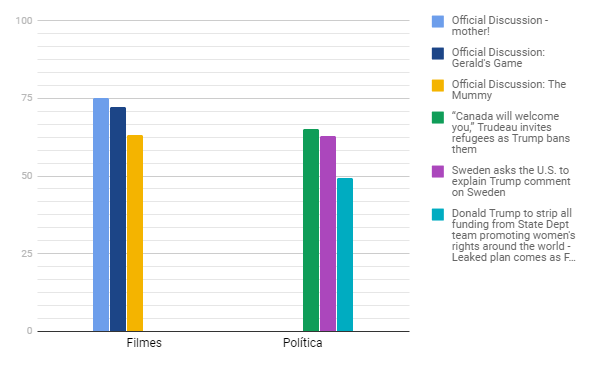
\includegraphics[height=300px]{imagens/grafico1.png}
\caption{Assertividade da ferramenta desenvolvida.}
\label{fig:ass}
\end{figure}